\documentclass{article}
\usepackage[utf8]{inputenc}

\title{Market View Report\\
        International Finance}

\author{Krish Gupta s3865829}   

\usepackage{natbib}
\usepackage{graphicx}
\usepackage{booktabs}
\usepackage{placeins}

\let\Oldsubsection\subsection
\renewcommand{\subsection}{\FloatBarrier\Oldsubsection}

\let\Oldsubsubsection\subsubsection
\renewcommand{\subsubsection}{\FloatBarrier\Oldsubsubsection}


\begin{document}
\maketitle

\tableofcontents
\pagebreak

\section*{Executive Summary}
\addcontentsline{toc}{section}{Executive Summary}
The report comprehensively analyses four key currency pairs: AUD/USD, USD/JPY, EUR/USD, and GBP/USD. We utilise the Fundamental approach for quantitative forecasting; qualitative data, such as inflation trends and public sentiment, further substantiate the report. The analysis indicates that the Australian Dollar and Japanese Yen are less likely to appreciate against the U.S. Dollar. In contrast, the Euro and British pound are poised for growth. Accordingly, the report advises an investment strategy favouring the Euro and British Pound while recommending the liquidation of the Australian Dollar and Japanese Yen assets.

\section*{Market View}
\addcontentsline{toc}{section}{Market View}

\subsection*{AUD/USD}
\addcontentsline{toc}{subsection}{AUD/USD}

Our analysis of various forecasting models—Random Walk (Appendix 1), Fundamental (Appendix 2), and Technical (Appendix 3)—reveals that the Fundamental approach is the most reliable for predicting trading rates, with the lowest standard deviation of approximately 0.33. Our latest forecast suggests the Australian dollar will not appreciate against the US dollar, predicting a max charge of \$0.769 by September 2023.

\begin{figure}[h!]
    \centering
    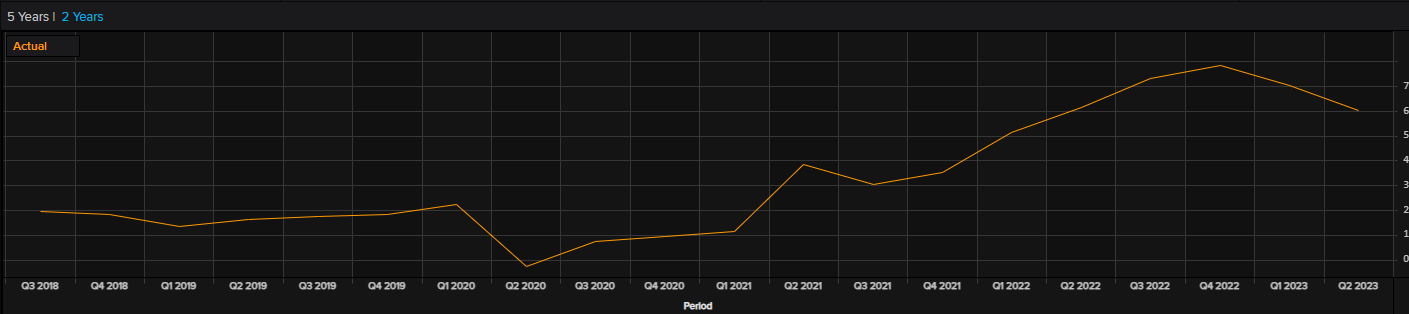
\includegraphics[scale=0.35]{graphs/AUDinflation-historical.png}
    \caption{Australian Historical Inflation Rate}
    \label{Australian Historical Inflation Rate}
\end{figure}



\noindent We also assessed inflation trends. Australia's inflation peaked at 7.8\% in Q4 of FY2022 but still falls within the Reserve Bank of Australia's 2-3\% target range. 

\begin{figure}[h!]
    \centering
    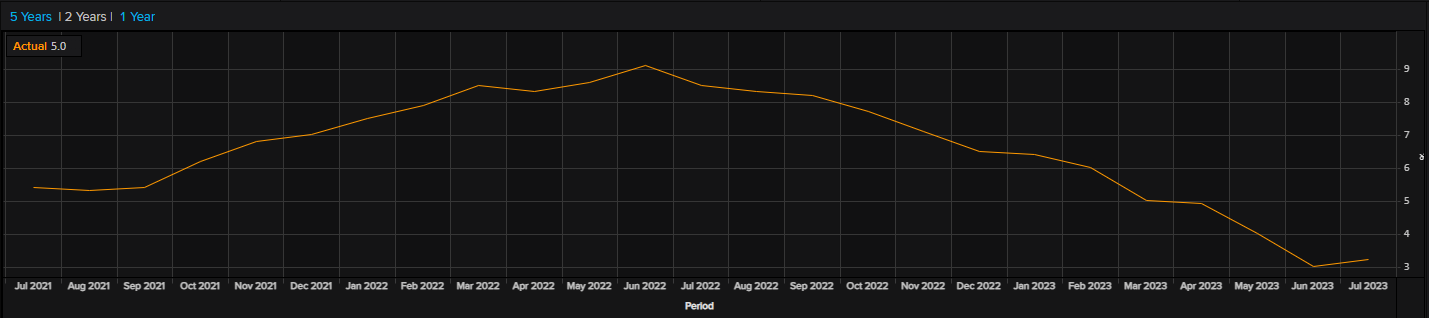
\includegraphics[scale=0.35]{graphs/USDinflation-historical.png}
    \caption{American Historical Inflation Rate}
    \label{American Historical Inflation Rate}
\end{figure}

\noindent Conversely, the US experienced a higher peak inflation of around 9\% in Q4 of FY2021 but recovered more quickly, dropping to 3\% in Q1 of FY2023. Australia's rate remains high at 6\%, and forecasts indicate a slower recovery than the US.\\

\begin{figure}[h!]
    \centering
    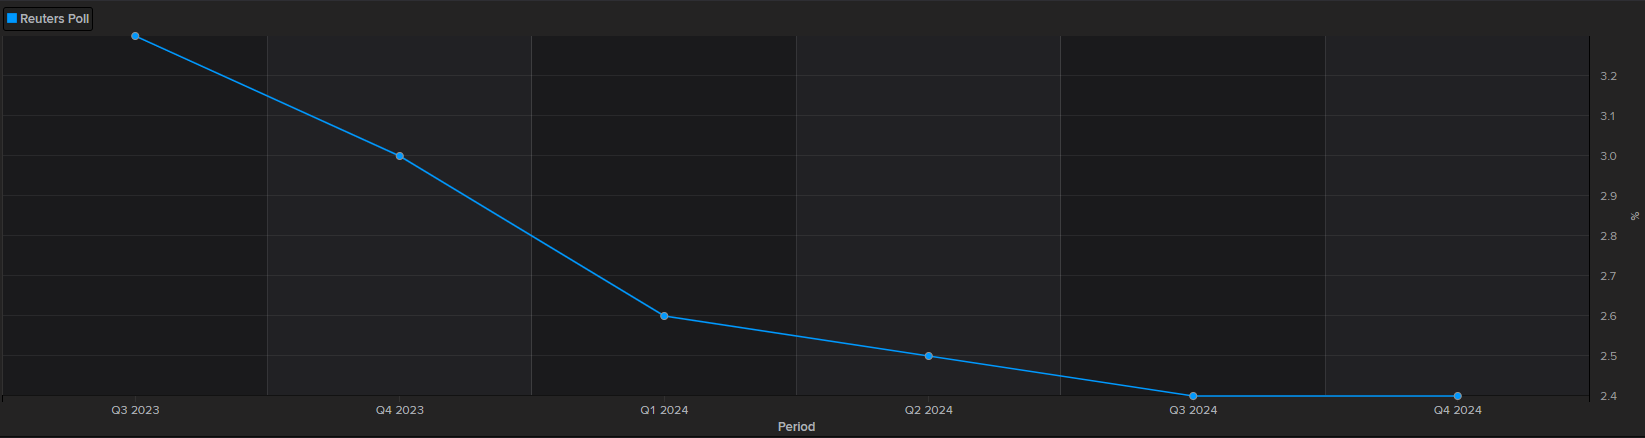
\includegraphics[scale=0.3]{graphs/USDinflation-forecast.png}
    \caption{American Forecasted Inflation Rate}
    \label{American Forecasted Inflation Rate}
\end{figure}

\begin{figure}[h!]
    \centering
    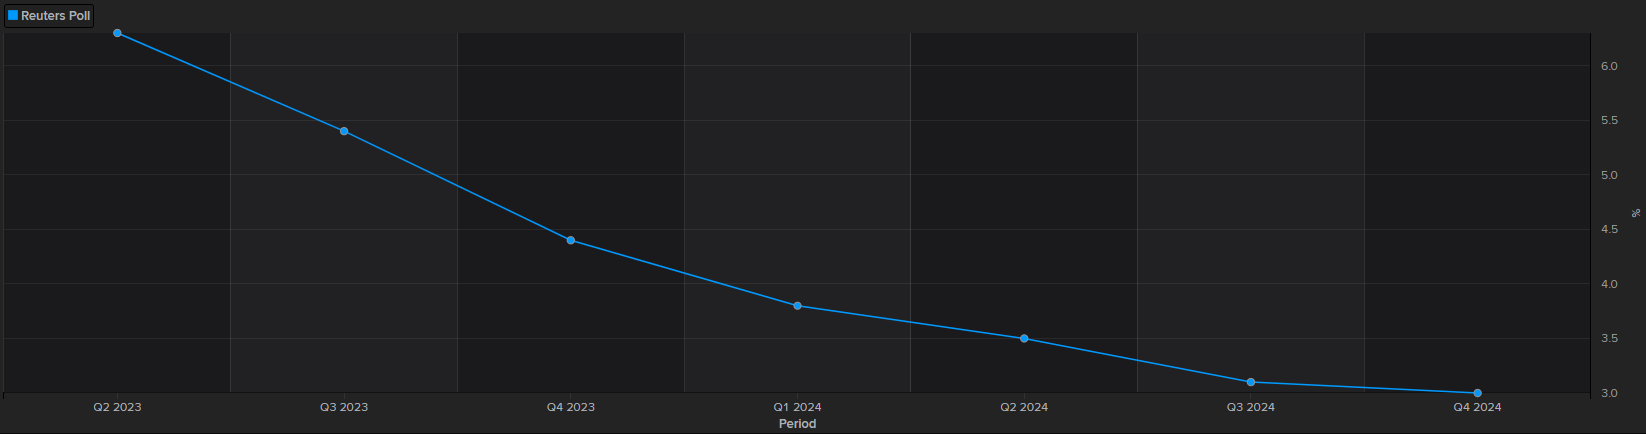
\includegraphics[scale=0.3]{graphs/AUDinflation-forecast.png}
    \caption{Australian Forecasted Inflation Rate}
    \label{Australian Forecasted Inflation Rate}
\end{figure}

\noindent High inflation tends to devalue a currency, reducing its purchasing power. Based on the higher and more prolonged inflation rates in Australia compared to the US, we expect the USD to continue appreciating against the AUD in the long run.

\subsection*{USD/JPY}
\addcontentsline{toc}{subsection}{USD/JPY}

After thoroughly analysing forecasting models—Random Walk (Appendix 4), Fundamental (Appendix 5), and Technical (Appendix 6)—we found the Fundamental approach to be the most reliable for predicting trading rates, with the lowest standard deviation of 2.44. Our latest projection suggests the Japanese Yen is unlikely to appreciate against the US dollar in the short term. 

\noindent Recent developments highlight Yen's nine-month low against the dollar, prompting Japan's Finance Minister to monitor market activities closely. Despite this, Japan's 3.4\% inflation rate closely mirrors the US rate, and long-term forecasts show a decline to 1.8\% by Q3 2024, potentially bolstering the Yen's future strength.

\begin{figure}[h!]
    \centering
    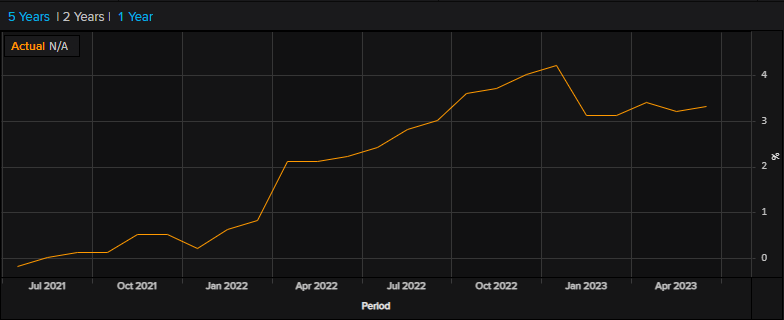
\includegraphics[scale=0.5]{graphs/JPY-CPI.png}
    \caption{Japan Historical Inflation Rate}
    \label{Japan Historical Inflation Rate}
\end{figure}

\begin{figure}[h!]
    \centering
    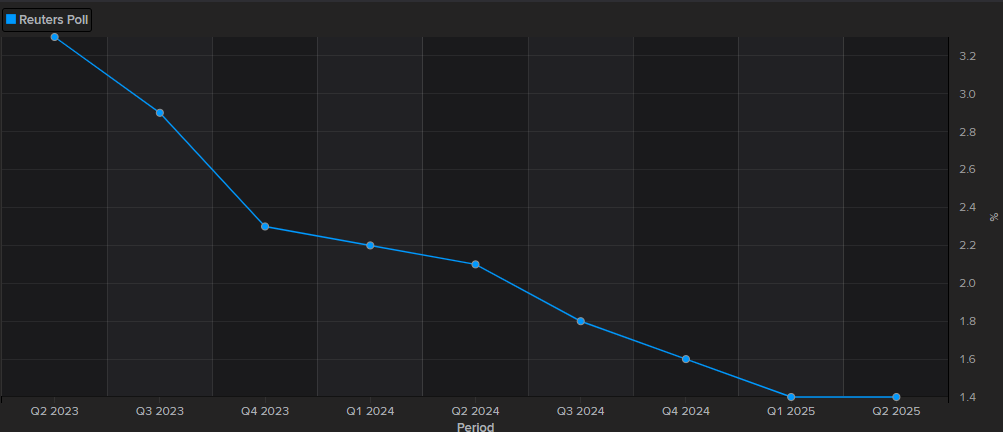
\includegraphics[scale=0.4]{graphs/JPY-forecastedCPI.png}
    \caption{Japan Forecasted Inflation Rate}
    \label{Japan Forecasted Inflation Rate}
\end{figure}

\noindent Japan's GDP growth aligns with OECD expectations, suggesting a possible economic rebound.

\begin{figure}[h!]
    \centering
    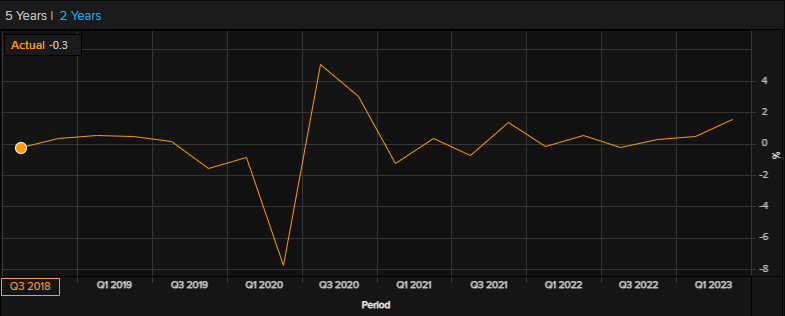
\includegraphics[scale=0.5]{graphs/JPY-GDP.png}
    \caption{Japan GDP}
    \label{Japan GDP}
\end{figure}

\noindent Given contrasting public sentiments and the US's looming inflation and a potential recession, the Yen shows signs of future appreciation. However, for the next month, the USD is expected to outperform the JPY.

\subsection*{EUR/USD}
\addcontentsline{toc}{subsection}{EUR/USD}
Our exhaustive evaluation of various forecasting models, such as Random Walk (Appendix 7), Fundamental (Appendix 8), and Technical (Appendix 9), indicates that the Fundamental approach is the most robust for predicting trading session rates, with the lowest standard deviation of 1.952. Our latest forecast suggests that the Euro will likely appreciate against the US dollar soon. 

\noindent A recent CNBC article corroborates this, reporting that the European Central Bank warns of sustained higher inflation in the Eurozone, which could indicate a looming recession. Current Eurozone GDP growth lags behind the U.S., at 2.3\% compared to 2.6\%, implying weaker demand for Eurozone products. 

\begin{figure}[h!]
    \centering
    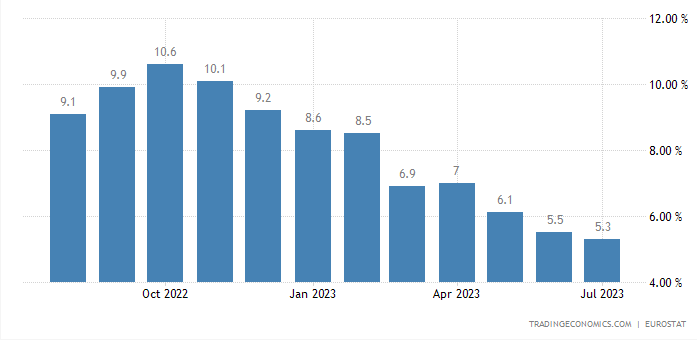
\includegraphics[scale=0.5]{graphs/EUR- Inflation Historical.png}
    \caption{Euro zone Inflation Rate}
    \label{Euro zone Inflation Rate}
\end{figure}

\begin{figure}[h!]
    \centering
    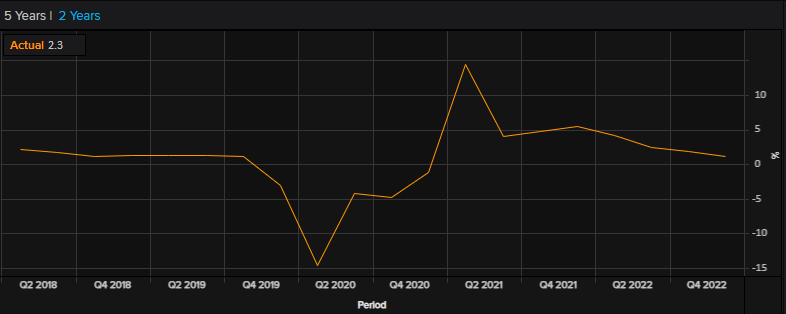
\includegraphics[scale=0.5]{graphs/Eur-GDP.png}
    \caption{Euro zone GDP}
    \label{Euro zone GDP}
\end{figure}

\begin{figure}[h!]
    \centering
    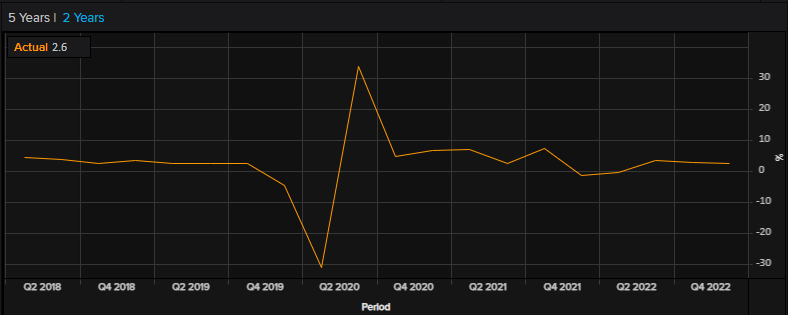
\includegraphics[scale=0.5]{graphs/Us-GDP.png}
    \caption{United States of America GDP}
    \label{United States of America GDP}
\end{figure}

\noindent However, the combination of persistently high inflation rates and positive public sentiment towards the Eurozone's swifter economic recovery is applying upward pressure on the value of the EUR relative to the USD. Given these factors, we concur with the article's forecast, anticipating the Euro to appreciate against the US dollar during our trading session.

\subsection*{GBP/USD}
\addcontentsline{toc}{subsection}{GBP/USD}
Our in-depth analysis of forecasting models—Random Walk (Appendix 10), Fundamental (Appendix 11), and Technical (Appendix 12)—indicates that the Fundamental approach is the most reliable for predicting trading session rates. It reports the lowest standard deviation of 2.396, contrasting with the other models' higher figures. Our latest forecast predicts the British Pound will appreciate against the US dollar, expecting a maximum charge of \$1.25 by September 2023.
\noindent A recent article by Christopher Lewis on August 18, 2023, supports this, noting the Pound's consecutive weeks of outperforming the dollar. Despite currency market volatility, the Pound exhibits a stable upward trend, buoyed by positive public sentiment and indicators like a 5\% rise in UK business investment this quarter. This bullish trend makes it an opportune moment for traders to leverage the Pound's strength to buy more USD.
\begin{figure}[h!]
    \centering
    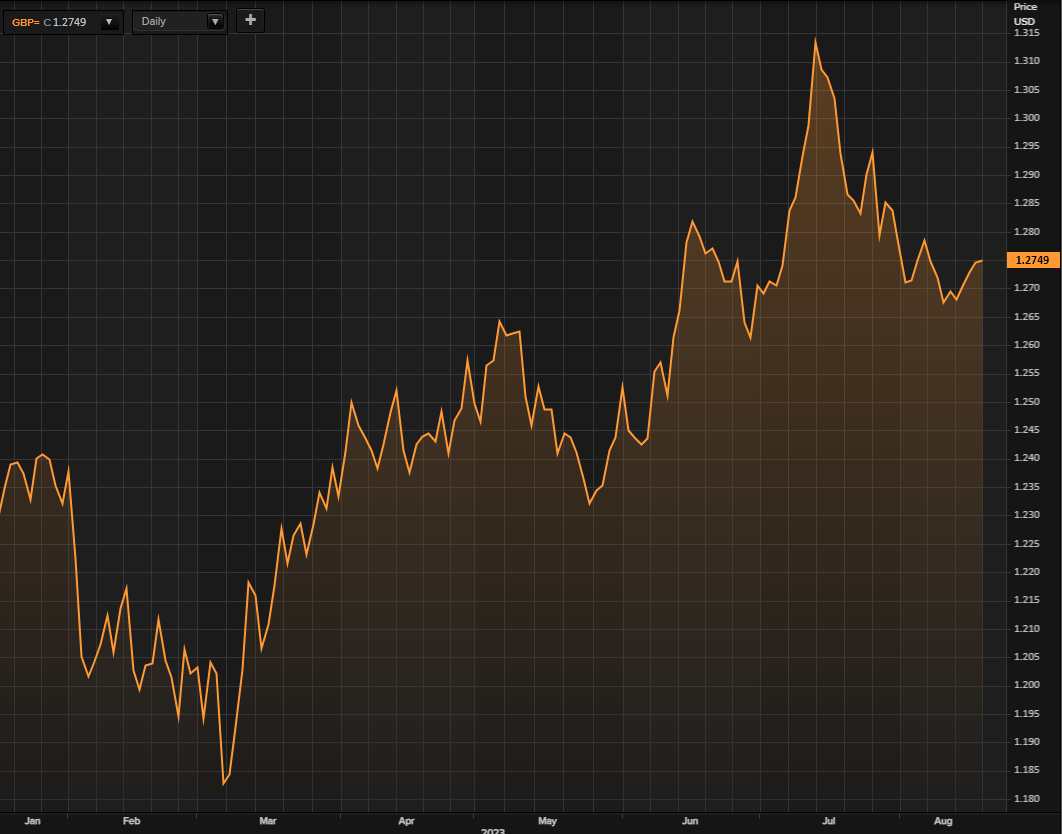
\includegraphics[scale=0.35]{graphs/GBP-SpotRate.png}
    \caption{GBP/USD Currency rate}
    \label{GBP/USD Currency rate}
\end{figure}

\FloatBarrier

\noindent Given the empirical and qualitative evidence, we forecast continued appreciation of the GBP against the USD in our investment timeframe.

\section*{Target Portfolio}
\addcontentsline{toc}{section}{Target Portfolio}

Based on our analysis, the U.S. Dollar is projected to gain strength against both the Australian Dollar (AUD) and the Japanese Yen (JPY). Given this forecast, we recommend structuring our target investment portfolio to favour the Euro (EUR) and the British Pound (GBP). Specifically, the British Pound is expected to appreciate notably against the U.S. Dollar, offering a significant opportunity for profit maximization.\\

\noindent Investing in the Euro and British Pound is strategically advantageous because these currencies currently exhibit higher purchasing power in the foreign exchange market. By converting our assets from USD to EUR and GBP, we stand to benefit from their projected strength.\\

\noindent We advise against acquiring AUD and JPY, given our anticipation that the U.S. Dollar will appreciate against these currencies. Consequently, it would be prudent to liquidate existing holdings in AUD and JPY to capitalize on the predicted currency movements.

\section*{Proposed Target Strategies}
\addcontentsline{toc}{section}{Proposed Target Strategies}
To achieve our target portfolio, we plan to liquidate our holdings in the Australian Dollar (AUD) and the Japanese Yen (JPY), converting these assets into U.S. Dollars (USD). These conversions will be executed through substantial transactions, each amounting to USD 10,000,000. While conducting trades of this magnitude carries a high level of risk and volatility, the robustness of our analysis gives us confidence that, when executed with precision, these moves will optimize our profit potential.\\

\noindent Upon securing a large pool of U.S. Dollars, we will invest in the Euro (EUR) and the British Pound (GBP). Transactions will also be capped at USD 10,000,000 but with a heavier allocation toward GBP. Our analysis indicates that the British Pound offers a more significant profit margin than the Euro. This investment strategy will continue either until the trading session concludes or until we have exhausted our supply of U.S. Dollars for trading.

\break

\section*{Appendix}
\addcontentsline{toc}{section}{Appendix}

\subsection*{AUD/USD Quantitative Analysis}
\addcontentsline{toc}{subsection}{AUD/USD Quantitative Analysis}

\subsection*{Appendix 1- Random Walk}


\begin{figure}[h!]
    \centering
    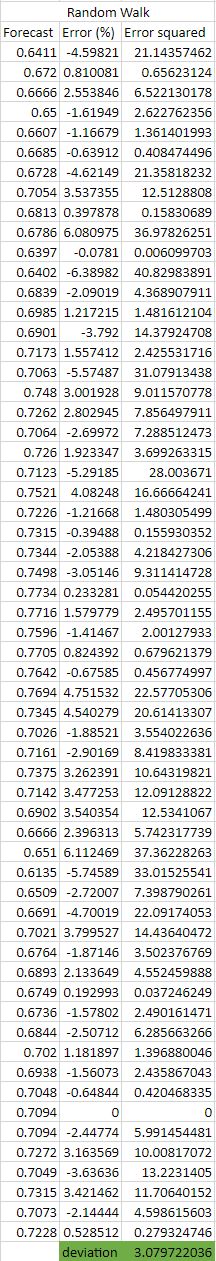
\includegraphics[scale=0.5]{graphs/appendix1.png}
\end{figure}

\break

\subsection*{Appendix 2- Fundamental Approach}


\begin{figure}[h!]
    \centering
    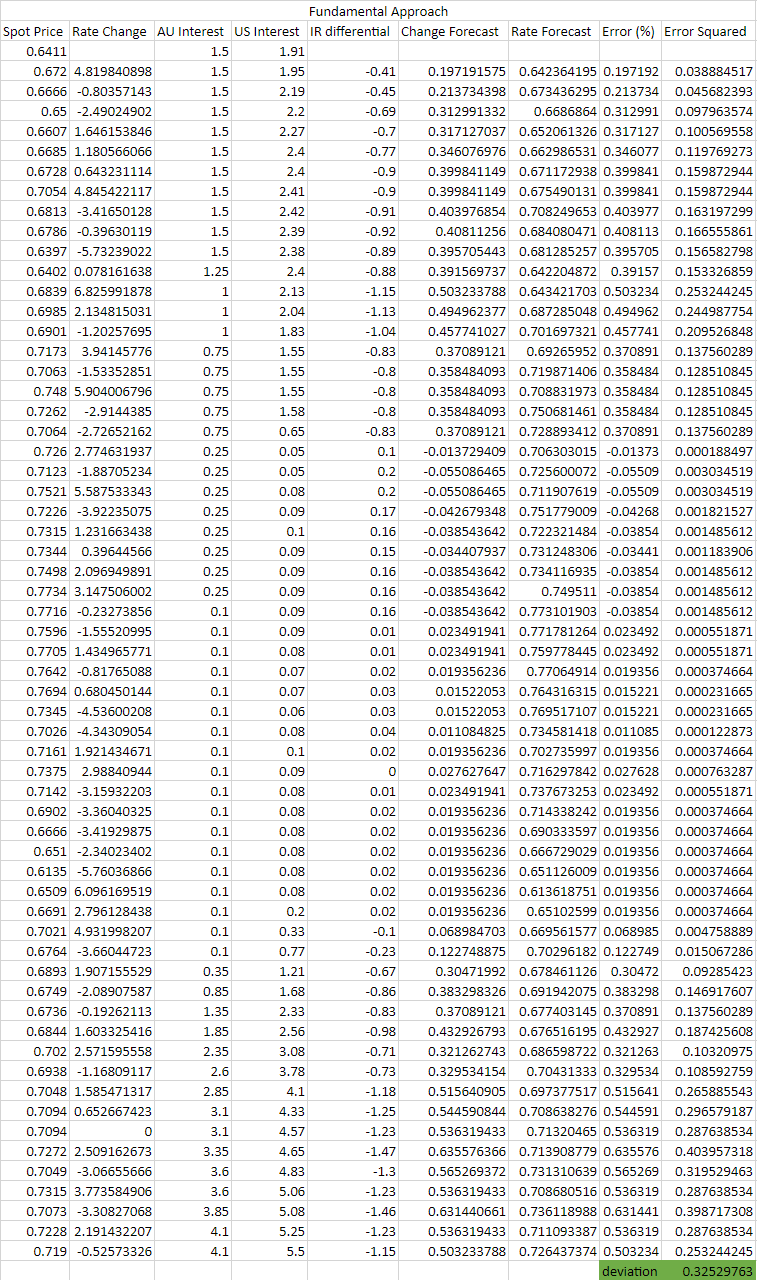
\includegraphics[scale=0.5]{graphs/appendix2-Fundamentals.png}
\end{figure}


\begin{figure}[h!]
    \centering
    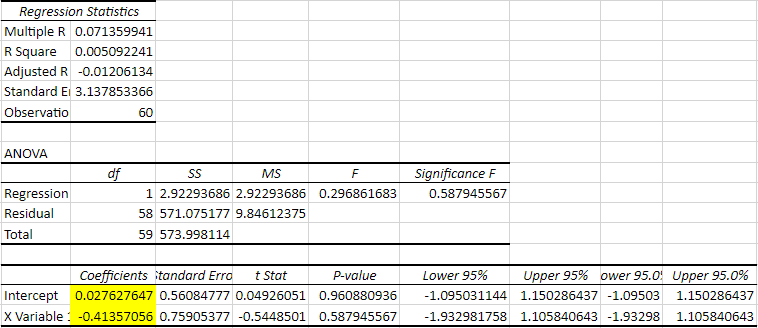
\includegraphics[scale=0.5]{graphs/appendix2-FunReg.png}
\end{figure}


\break


\subsection*{Appendix 3- Technical Approach}
\begin{figure}[h!]
    \centering
    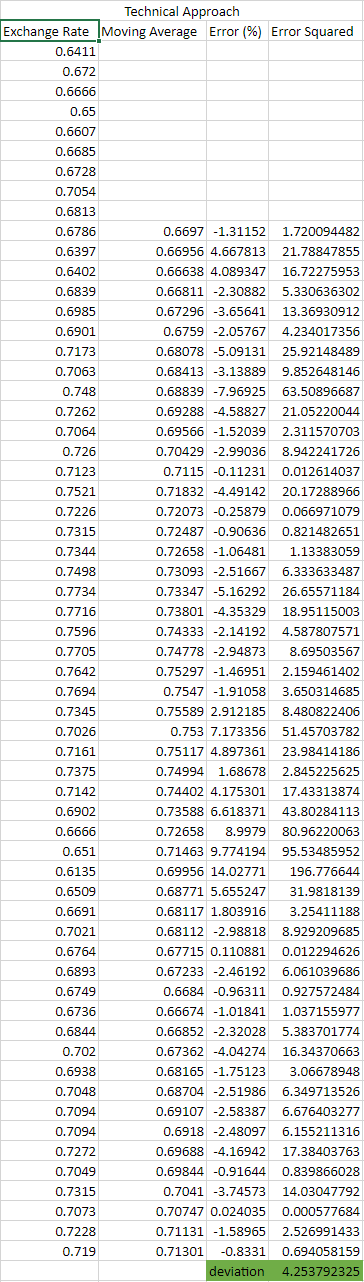
\includegraphics[scale=0.5]{graphs/appendix3-Technical.png}
\end{figure}

\FloatBarrier
\subsection*{USD/JPY Quantitative Analysis}
\addcontentsline{toc}{subsection}{USD/JPY Quantitative Analysis}

\subsection*{Appendix 4- Random Walk}


\begin{figure}[h!]
    \centering
    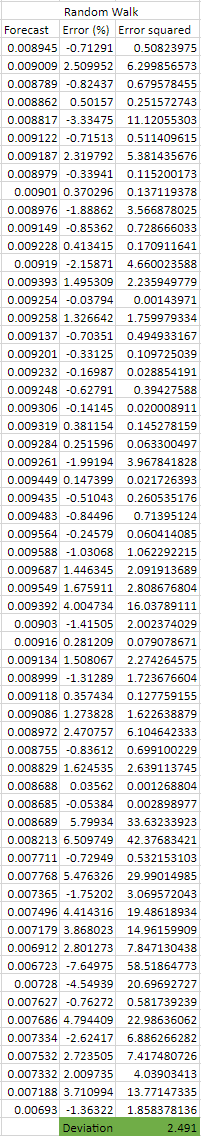
\includegraphics[scale=0.5]{graphs/app4.png}
\end{figure}

\break

\subsection*{Appendix 5- Fundamental Approach}


\begin{figure}[h!]
    \centering
    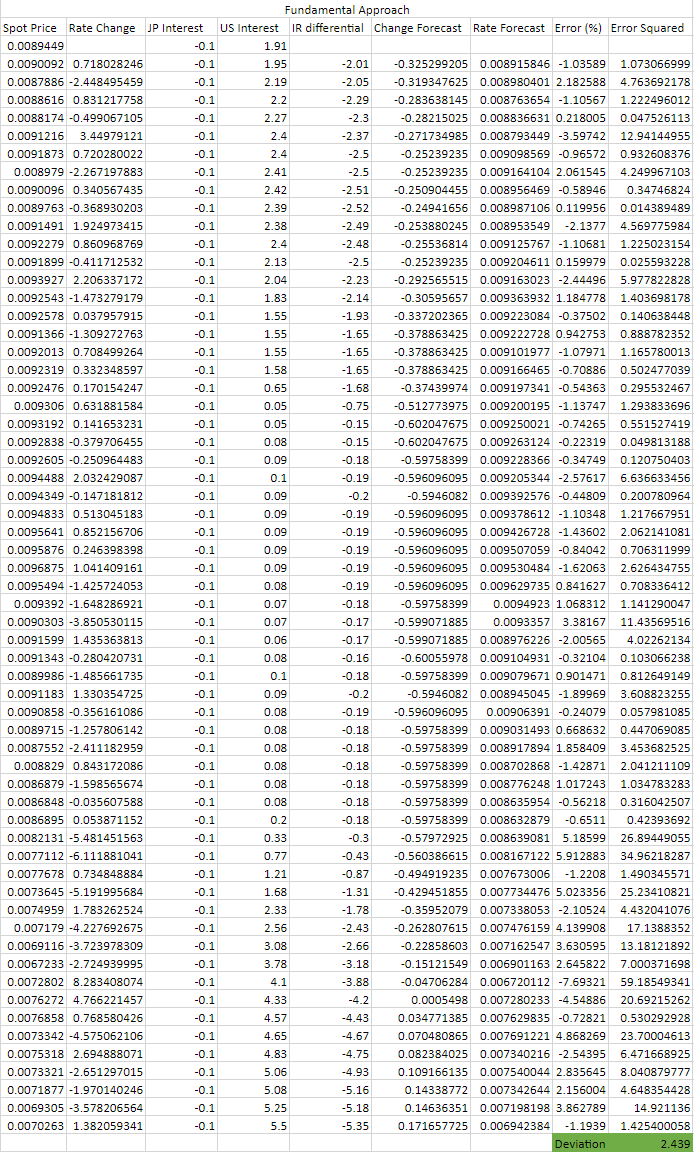
\includegraphics[scale=0.5]{graphs/app5.png}
\end{figure}


\begin{figure}[h!]
    \centering
    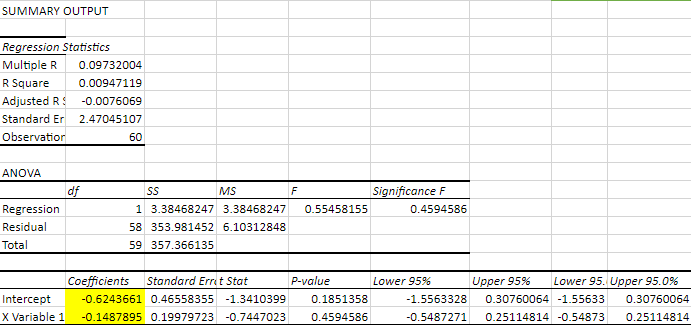
\includegraphics[scale=0.5]{graphs/app5(1).png}
\end{figure}

\break

\subsection*{Appendix 6- Technical Approach}


\begin{figure}[h!]
    \centering
    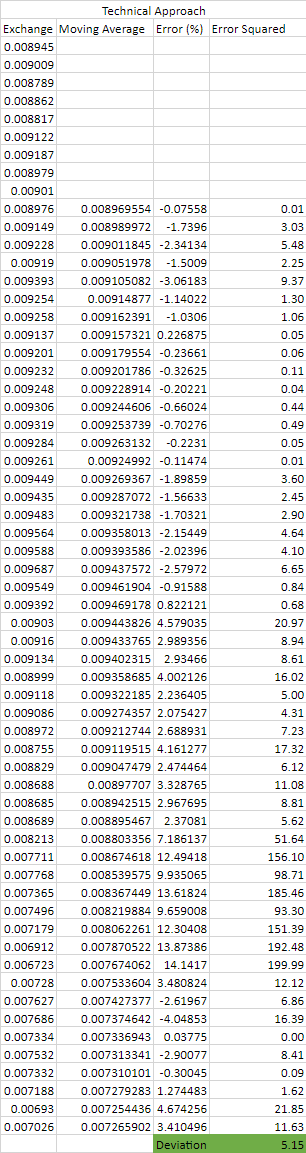
\includegraphics[scale=0.5]{graphs/app6.png}
\end{figure}

\subsection*{EUR/USD Quantitative Analysis}
\addcontentsline{toc}{subsection}{EUR/USD Quantitative Analysis}

\subsection*{Appendix 7- Random Walk}


\begin{figure}[h!]
    \centering
    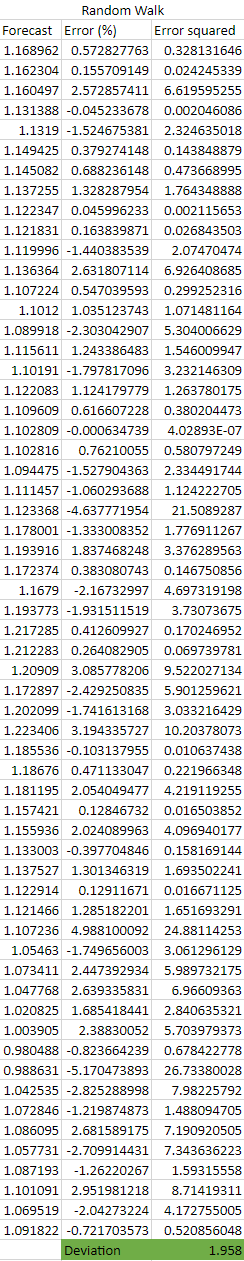
\includegraphics[scale=0.5]{graphs/app7.png}
\end{figure}

\break

\subsection*{Appendix 8- Fundamental Approach}


\begin{figure}[h!]
    \centering
    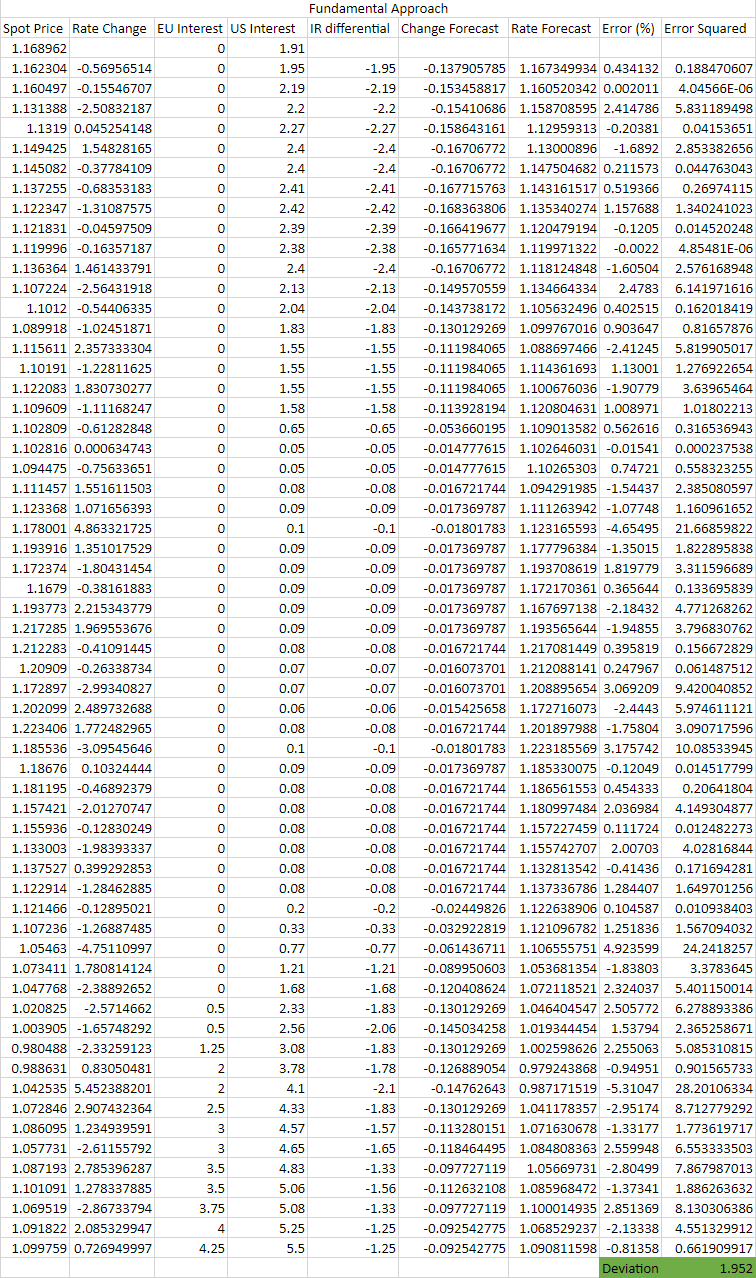
\includegraphics[scale=0.5]{graphs/app8.png}
\end{figure}


\begin{figure}[h!]
    \centering
    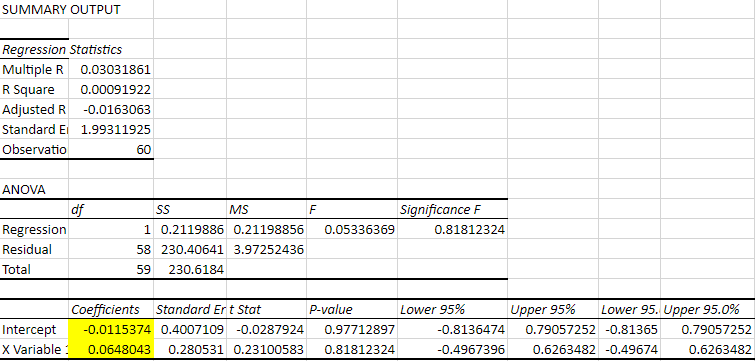
\includegraphics[scale=0.5]{graphs/app8(1).png}
\end{figure}

\break

\subsection*{Appendix 9- Technical Approach}


\begin{figure}[h!]
    \centering
    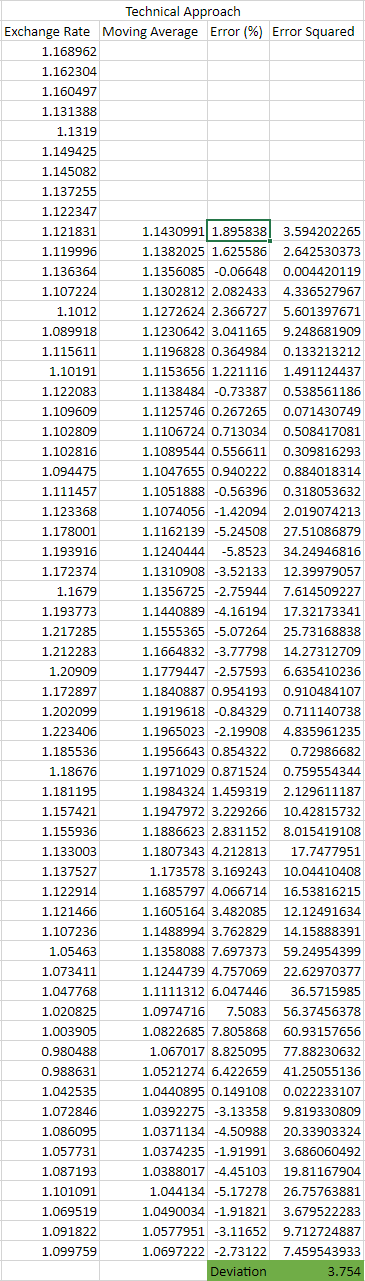
\includegraphics[scale=0.5]{graphs/app9.png}
\end{figure}

\subsection*{GBP/USD Quantitative Analysis}
\addcontentsline{toc}{subsection}{GBP/USD Quantitative Analysis}

\subsection*{Appendix 10- Random Walk}


\begin{figure}[h!]
    \centering
    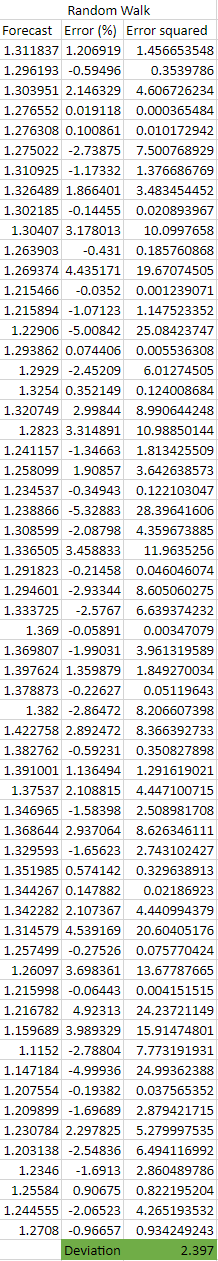
\includegraphics[scale=0.5]{graphs/app10.png}
\end{figure}

\break

\subsection*{Appendix 11- Fundamental Approach}


\begin{figure}[h!]
    \centering
    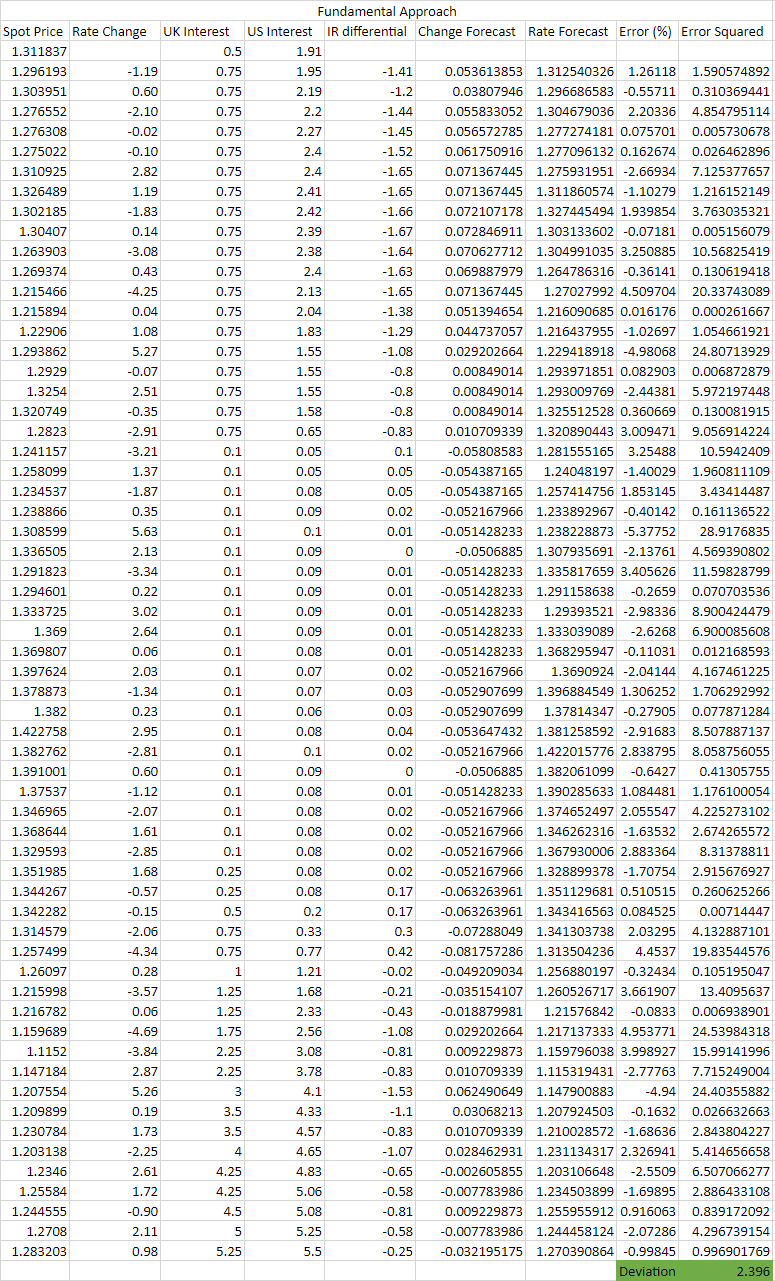
\includegraphics[scale=0.5]{graphs/app11.png}
\end{figure}


\begin{figure}[h!]
    \centering
    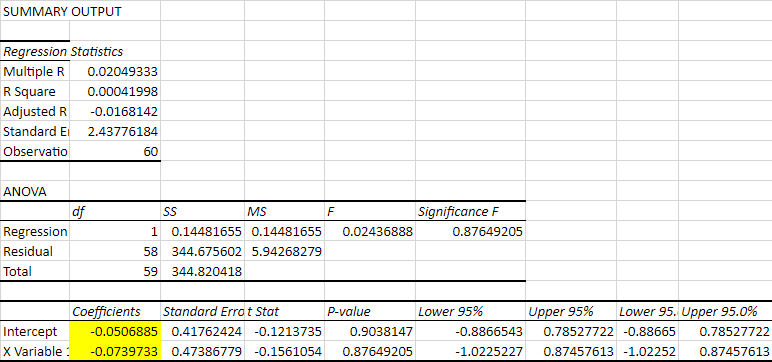
\includegraphics[scale=0.5]{graphs/app11(1).png}
\end{figure}

\subsection*{Appendix 12- Technical Approach}
\begin{figure}[h!]
    \centering
    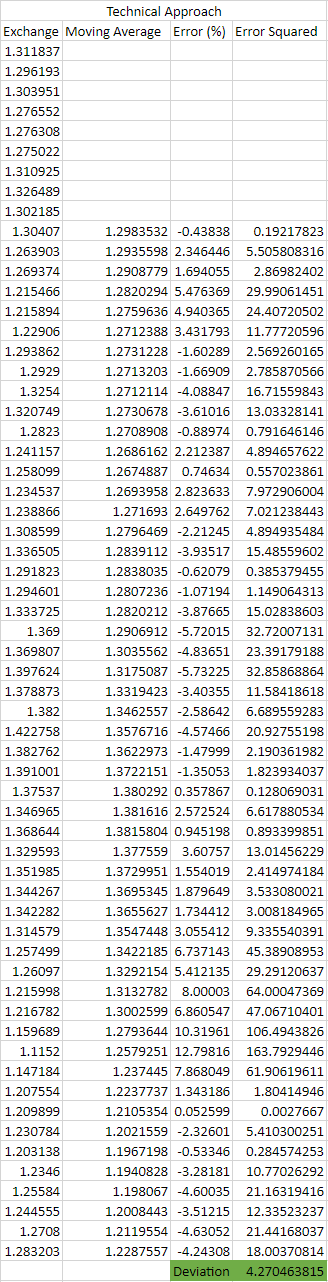
\includegraphics[scale=0.5]{graphs/app12.png}
\end{figure}

\FloatBarrier

\section*{References}
\addcontentsline{toc}{section}{References}




\end{document}  